%========================================================
% CHAPTER 3 — Physical and Mathematical Representation
%========================================================

\chapter{Physical and Mathematical Representation}

%========================================================
% SECTION 3.1 — Quantum System and Hilbert Space Structure
%========================================================

\section{Quantum System and Hilbert Space Structure}

The physical system considered consists of polarization-entangled photon pairs generated by spontaneous parametric down-conversion (SPDC). The two photons propagate along distinct optical paths, denoted \( A \) and \( B \), forming a bipartite quantum system.

\medskip

In this work, the qubit is encoded in the polarization degree of freedom:

\begin{equation}
|H\rangle \equiv |0\rangle,
\qquad
|V\rangle \equiv |1\rangle.
\label{eq:polarization_computational_encoding}
\end{equation}

Accordingly, the computational basis of the bipartite system is

\begin{equation}
\mathcal{B}_{AB}
=
\{
|00\rangle,\,
|01\rangle,\,
|10\rangle,\,
|11\rangle
\}.
\label{eq:two_qubit_computational_basis}
\end{equation}

In polarization notation, this corresponds to

\[
\{
|H\rangle_A |H\rangle_B,\,
|H\rangle_A |V\rangle_B,\,
|V\rangle_A |H\rangle_B,\,
|V\rangle_A |V\rangle_B
\}.
\]

\medskip

The Hilbert space of the total system is therefore

\begin{equation}
\mathcal{H}_{AB}
=
\mathcal{H}_A \otimes \mathcal{H}_B
\simeq
\mathbb{C}^{2} \otimes \mathbb{C}^{2}.
\label{eq:two_qubit_hilbert_space}
\end{equation}

Since each subsystem is two-dimensional, the composite Hilbert space has dimension \(4\).

As a consequence:
\begin{itemize}
    \item pure states are represented by complex vectors of length \(4\),
    \item operators acting on the full bipartite system are represented by \(4 \times 4\) matrices.
\end{itemize}

\medskip

This construction provides a concrete realization of the quantum-information framework introduced above.

The fixed computational basis in Eq.~\eqref{eq:two_qubit_computational_basis} will be used consistently throughout the theoretical development, the numerical implementation, and the validation experiments.

%========================================================
% SECTION 3.2 — Bell-State Initialization
%========================================================

\section{Bell-State Initialization}

As a reference initial condition, this work considers the Bell state

\begin{equation}
|\Psi^{+}\rangle
=
\frac{1}{\sqrt{2}}
\left(
|H\rangle_A |V\rangle_B
+
|V\rangle_A |H\rangle_B
\right).
\label{eq:bell_psi_plus_polarization}
\end{equation}

Using the computational-basis convention introduced in Eq.~\eqref{eq:polarization_computational_encoding}, the same state can be written as

\begin{equation}
|\Psi^{+}\rangle
=
\frac{1}{\sqrt{2}}
\left(
|01\rangle + |10\rangle
\right).
\label{eq:bell_psi_plus}
\end{equation}

\medskip

In the ordered computational basis \( \mathcal{B}_{AB} \), this state is represented by the column vector

\begin{equation}
|\Psi^{+}\rangle
=
\frac{1}{\sqrt{2}}
\begin{pmatrix}
0\\
1\\
1\\
0
\end{pmatrix}.
\label{eq:bell_psi_plus_vector}
\end{equation}

\medskip

The state \( |\Psi^+\rangle \) is maximally entangled and provides the natural input for the baseline version of the simulator. It also serves as the reference state with respect to which later quantities such as fidelity and Bell-inequality violation may be evaluated.

\medskip

The Bell state provides both a clean analytical benchmark and a physically relevant entangled resource, enabling direct interpretation of fiber-induced effects in terms of coherence, two-photon correlations, and nonlocality.

\medskip

For completeness, the four Bell states are

\begin{equation}
|\Psi^{\pm}\rangle
=
\frac{1}{\sqrt{2}}
\left(
|01\rangle \pm |10\rangle
\right),
\qquad
|\Phi^{\pm}\rangle
=
\frac{1}{\sqrt{2}}
\left(
|00\rangle \pm |11\rangle
\right).
\label{eq:bell_state_basis}
\end{equation}

Among these, \( |\Psi^+\rangle \) is used as the default reference input for the propagation models considered in this work.

%========================================================
% SECTION 3.3 — Fiber Propagation as Local Unitary Evolution
%========================================================

\section{Fiber Propagation as Local Unitary Evolution}

Each photon propagates through its own optical fiber. At the level of the polarization qubit, the action of each fiber is described by a linear operator acting locally on the corresponding single-photon Hilbert space. In the ideal lossless description, this operator is unitary.

\medskip

If \( U_A \) and \( U_B \) denote the single-qubit operators associated with the two fibers, the evolution of an initial two-photon state is

\begin{equation}
|\psi_{\mathrm{out}}\rangle
=
(U_A \otimes U_B)
|\psi_{\mathrm{in}}\rangle.
\label{eq:local_unitary_state_evolution}
\end{equation}

\medskip

This expression follows directly from the tensor-product structure of composite quantum systems and represents the natural bipartite extension of single-qubit evolution. It provides the fundamental starting point for subsequent refinements, including random unitary perturbations, concatenated fiber sections, and effective channel descriptions.

\medskip

In this framework, the two fibers act independently on the two polarization subsystems, and the total evolution is obtained by tensor composition of the corresponding local transformations. This description remains valid as long as the fibers do not induce any direct interaction between the two photons.

\medskip

The local-unitary model is therefore the first dynamical layer of the thesis: it captures deterministic polarization transformations while preserving the purity of the global two-photon state.

%========================================================
% SECTION 3.4 — Pure-State and Density-Operator Descriptions
%========================================================

\section{Pure-State and Density-Operator Descriptions}
\label{sec:pure_state_and_density_operator_descriptions}

The first modeling level describes the two-photon system as a pure state in the bipartite Hilbert space
\( \mathbb{C}^2 \otimes \mathbb{C}^2 \). In this regime, fiber propagation is represented by local unitary transformations acting independently on the two polarization qubits.

\medskip

As introduced in Eq.~\eqref{eq:local_unitary_state_evolution}, the evolution remains fully coherent and deterministic, with the quantum state being represented directly through a state vector
\( |\psi\rangle \).

\medskip

A more general and operationally complete description is obtained through the density operator formalism. For a pure bipartite state \( |\psi\rangle \), the associated density operator is defined as

\begin{equation}
\rho_{AB}
=
|\psi\rangle\langle\psi| .
\label{eq:pure_state_density_operator}
\end{equation}

The density operator \( \rho_{AB} \) contains the complete statistical and physical information associated with the quantum state. In the pure-state regime, Eq.~\eqref{eq:pure_state_density_operator} is fully equivalent to the vector representation, since both descriptions encode the same physical state.

\medskip

The density-operator formalism, however, extends naturally beyond pure states and therefore provides the appropriate framework for the subsequent modeling levels developed throughout this work. In particular, it becomes necessary when introducing:

\begin{itemize}
    \item statistical ensembles of quantum states,
    \item reduced subsystem descriptions obtained through partial traces,
    \item effective non-unitary evolution induced by noisy channels,
    \item mixed states arising from decoherence and depolarization.
\end{itemize}

\medskip

For this reason, although the initial propagation models can be formulated entirely at the pure-state level, the density-operator representation will progressively become central in the mathematical framework and in the quantitative analyses developed in the following chapters.

%--------------------------------------------------------
% Subsection 3.4.1 — Reduced Density Operators
%--------------------------------------------------------

\subsection{Reduced Density Operators}
\label{subsec:reduced_density_operators}

A central operation in the density-operator formalism is the partial trace. It allows one to describe the state accessible to a single subsystem when the global bipartite system is described by \( \rho_{AB} \).

\medskip

The reduced density operators are defined as

\begin{equation}
\rho_A
=
\mathrm{Tr}_B(\rho_{AB}),
\qquad
\rho_B
=
\mathrm{Tr}_A(\rho_{AB}).
\end{equation}

These operators contain all information accessible through local measurements on the corresponding subsystem. For any observable \( O_A \) acting only on arm \( A \),

\begin{equation}
\langle O_A \rangle
=
\mathrm{Tr}
\left[
\rho_{AB}
\left(
O_A \otimes I_B
\right)
\right]
=
\mathrm{Tr}(\rho_A O_A).
\end{equation}

\medskip

An explicit expression for the partial trace over subsystem \( B \) is

\begin{equation}
\rho_A
=
\sum_{j=0}^{1}
\left(
I_A \otimes \langle j|
\right)
\rho_{AB}
\left(
I_A \otimes |j\rangle
\right),
\end{equation}

where \( \{|0\rangle, |1\rangle\} \) is the computational basis of subsystem \( B \). The analogous expression defines \( \rho_B \) by tracing over subsystem \( A \).

\medskip

For the Bell state

\[
|\Psi^+\rangle
=
\frac{1}{\sqrt{2}}
\left(
|01\rangle + |10\rangle
\right),
\]

the reduced states are maximally mixed:

\begin{equation}
\rho_A
=
\rho_B
=
\frac{1}{2}I.
\end{equation}

This result shows that each photon is locally unpolarized, even though the global two-photon state is pure and maximally entangled.

%--------------------------------------------------------
% Subsection 3.4.2 — Extension to Mixed-State Descriptions
%--------------------------------------------------------

\subsection{Extension to Mixed-State Descriptions}
\label{subsec:mixed_state_descriptions}

The density-operator formalism also describes states that cannot be represented by a single state vector. This situation appears when different realizations of the system are combined statistically, or when unresolved degrees of freedom are not modeled explicitly.

\medskip

A generic mixed state can be written as a convex combination

\begin{equation}
\rho
=
\sum_k q_k
|\psi_k\rangle\langle\psi_k|,
\qquad
q_k \geq 0,
\qquad
\sum_k q_k = 1.
\label{eq:mixed_state_convex_decomposition}
\end{equation}

In the context of fiber propagation, this representation is useful for describing random phase fluctuations. If each photon pair experiences a different phase realization \( \theta_k \), the ensemble state is

\begin{equation}
\rho_{AB}^{(\mathrm{ens})}
=
\sum_k q_k
|\psi(\theta_k)\rangle
\langle \psi(\theta_k)|.
\end{equation}

For a uniform numerical average over \( N \) sampled realizations, this becomes

\begin{equation}
\rho_{AB}^{(\mathrm{ens})}
=
\frac{1}{N}
\sum_{k=1}^{N}
|\psi(\theta_k)\rangle
\langle \psi(\theta_k)|.
\end{equation}

\medskip

The density-operator formalism is therefore the natural framework for describing statistical phase averaging, local reduced states, and later effective non-unitary dynamics through quantum channels.

%--------------------------------------------------------
% Subsection 3.4.3 — Expectation Values
%--------------------------------------------------------

\subsection{Expectation Values}
\label{subsec:density_operator_expectation_values}

In the pure-state formalism, the expectation value of an observable \( O \) is

\[
\langle O \rangle
=
\langle \psi | O | \psi \rangle .
\]

In the density-operator formalism, this expression generalizes to

\begin{equation}
\langle O \rangle
=
\mathrm{Tr}(\rho O).
\label{eq:density_expectation_value}
\end{equation}

This formula applies both to pure states and to mixed states. Indeed, for
\( \rho = |\psi\rangle\langle\psi| \), one recovers

\[
\mathrm{Tr}(\rho O)
=
\mathrm{Tr}
\left(
|\psi\rangle\langle\psi| O
\right)
=
\langle \psi | O | \psi \rangle .
\]

\medskip

This unified expression is used throughout the simulator to compute local quantities, state metrics, and two-photon observables from the same matrix-based representation.

%========================================================
% SECTION 3.5 — Reduced Phase Model
%========================================================

\section{Reduced Phase Model}
\label{sec:reduced_phase_model}

Although a general fiber transformation may involve arbitrary polarization rotations, birefringence, and mode-coupling effects, the first approximation adopted here is simpler and directly motivated by the experimental control scheme.

After partial compensation of polarization drifts, the dominant residual effect is modeled as a relative phase shift between the horizontal and vertical polarization components. In the qubit representation, this corresponds to an effective rotation around the computational \( Z \)-axis of the Bloch sphere.

\medskip

At the single-qubit level, this is represented by the diagonal unitary

\begin{equation}
U(\theta)
=
\begin{pmatrix}
1 & 0\\
0 & e^{i\theta}
\end{pmatrix},
\label{eq:single_qubit_phase_unitary}
\end{equation}

defined up to an irrelevant global phase.

\medskip

If the two fibers induce phases \( \theta_A \) and \( \theta_B \), the total transformation is

\begin{equation}
U_A \otimes U_B
=
U(\theta_A) \otimes U(\theta_B).
\label{eq:two_arm_phase_unitary}
\end{equation}

Applying this operator to the reference Bell state \( |\Psi^+\rangle \) yields

\begin{equation}
|\psi(\theta_A,\theta_B)\rangle
=
\frac{1}{\sqrt{2}}
\left(
e^{i\theta_B}|01\rangle
+
e^{i\theta_A}|10\rangle
\right).
\label{eq:two_phase_bell_state}
\end{equation}

The phase accumulated by each computational component depends on which subsystem carries the logical state \( |1\rangle \).
In particular, the component \( |01\rangle \) acquires the phase generated by subsystem \( B \), while the component \( |10\rangle \) acquires the phase generated by subsystem \( A \).

\medskip

Factoring out the global phase \( e^{i\theta_B} \), which has no observable effect, gives the reduced one-parameter state

\begin{equation}
|\psi(\theta)\rangle
=
\frac{1}{\sqrt{2}}
\left(
|01\rangle
+
e^{i\theta}|10\rangle
\right),
\qquad
\theta = \theta_A - \theta_B.
\label{eq:reduced_phase_bell_state}
\end{equation}

Consequently, only the relative phase difference between the two arms has physical significance.
Any common phase contribution acts as a global phase factor and therefore does not modify observable quantities.

\medskip

With the convention adopted throughout this work, the reduced state in Eq.~\eqref{eq:reduced_phase_bell_state} can be interpreted equivalently as arising from a local phase rotation acting only on subsystem \( A \),

\begin{equation}
U_A(\theta)
=
\begin{pmatrix}
1 & 0\\
0 & e^{i\theta}
\end{pmatrix},
\qquad
U_B = I,
\label{eq:single_arm_phase_convention}
\end{equation}

so that

\begin{equation}
(U_A \otimes I)|\Psi^+\rangle
=
\frac{1}{\sqrt{2}}
\left(
|01\rangle
+
e^{i\theta}|10\rangle
\right).
\label{eq:phase_convention_state}
\end{equation}

This convention is adopted for consistency across the analytical derivations and numerical implementation developed throughout the present work.

\medskip

\paragraph{Interpretation.}

In this reduced description, the physically relevant fiber action is encoded in a single parameter: the relative phase \( \theta \), determined by propagation conditions such as birefringence, path length, and environmental fluctuations.

The model isolates the dominant contribution affecting two-photon correlations while preserving a pure-state description. As a consequence, entanglement remains maximal and all observable variations arise from phase-induced modifications of quantum coherence.

\medskip

\paragraph{Role in the modeling hierarchy.}

The reduced phase model constitutes the first nontrivial propagation model in the hierarchy. It provides an analytically tractable reference case for validating the simulator and serves as the baseline for subsequent extensions, including general unitary dynamics, ensemble descriptions, and effective non-unitary evolutions.

%========================================================
% SECTION 3.6 — Correlation Tensor Representation
%========================================================

\section{Correlation Tensor Representation}
\label{sec:correlation_tensor_representation}

Bipartite correlations are described through the Pauli-operator basis

\[
\sigma_i \otimes \sigma_j,
\qquad
i,j \in \{x,y,z\},
\]

constructed from the single-qubit Pauli matrices \( \sigma_x, \sigma_y, \sigma_z \). It is also useful to introduce \( \sigma_0 = I \), so that local terms and correlations can be treated within a single notation.

\medskip

For a two-qubit state \( \rho_{AB} \), the expectation values

\begin{equation}
T_{ij}
=
\mathrm{Tr}
\left(
\rho_{AB}\,
\sigma_i \otimes \sigma_j
\right),
\qquad
i,j \in \{x,y,z\},
\label{eq:correlation_tensor_components}
\end{equation}

define the components of the correlation tensor \( T \in \mathbb{R}^{3 \times 3} \).

\medskip

More generally, the state admits the Pauli decomposition

\begin{equation}
\rho_{AB}
=
\frac{1}{4}
\sum_{i,j=0}^{3}
S_{ij}\,
\sigma_i \otimes \sigma_j,
\qquad
S_{ij}
=
\mathrm{Tr}
\left(
\rho_{AB}\,
\sigma_i \otimes \sigma_j
\right),
\label{eq:two_qubit_pauli_decomposition}
\end{equation}

where \( S_{ij} \) are generalized Stokes parameters. This representation is commonly used in quantum-state tomography of two-qubit photonic systems, where the density operator is reconstructed from measured expectation values of tensor products of Pauli operators~\cite{altepeter_james_kwiat_quantum_state_tomography}.

In this representation:
\begin{itemize}
    \item \( S_{i0} \) and \( S_{0j} \) encode the local Bloch vectors of the two subsystems,
    \item the block \( S_{ij} \), with \( i,j \in \{x,y,z\} \), corresponds to the correlation tensor \( T_{ij} \).
\end{itemize}

\medskip

The orthogonality relation

\begin{equation}
\mathrm{Tr}
\left[
(\sigma_i \otimes \sigma_j)
(\sigma_k \otimes \sigma_l)
\right]
=
4\,\delta_{ik}\delta_{jl}
\label{eq:pauli_tensor_orthogonality}
\end{equation}

ensures that all coefficients in Eq.~\eqref{eq:two_qubit_pauli_decomposition} are obtained by direct projection.

\medskip

\paragraph{Analytical behavior in the reduced phase model.}

For the phase-evolved Bell state in Eq.~\eqref{eq:reduced_phase_bell_state}, the correlation tensor is

\begin{equation}
T(\theta)
=
\begin{pmatrix}
\cos\theta & -\sin\theta & 0\\
\sin\theta & \cos\theta & 0\\
0 & 0 & -1
\end{pmatrix}.
\label{eq:correlation_tensor_phase_model}
\end{equation}

This structure shows that the parameter \( \theta \) induces a rotation in the transverse \( x\text{-}y \) correlation plane, while leaving the longitudinal \( z \)-component invariant.

\medskip

The commonly evaluated diagonal correlations are

\begin{align}
\langle \sigma_x \otimes \sigma_x \rangle
&=
T_{xx}
=
\cos\theta,
\nonumber
\\
\langle \sigma_y \otimes \sigma_y \rangle
&=
T_{yy}
=
\cos\theta,
\nonumber
\\
\langle \sigma_z \otimes \sigma_z \rangle
&=
T_{zz}
=
-1.
\label{eq:phase_model_diagonal_correlations}
\end{align}

\medskip

\paragraph{Interpretation.}

The reduced phase model modifies only coherence terms, producing a rigid rotation of correlations in the transverse plane. Population correlations remain unchanged, reflecting the purely unitary nature of the transformation.

The correlation tensor is therefore the natural object for distinguishing changes in measurement alignment from actual loss of quantum coherence or entanglement.

\medskip

\paragraph{Dependence on the local operator basis.}

The numerical values of the tensor components \( T_{ij} \) depend on the choice of local measurement axes used to define the Pauli operators.

Under local unitary transformations,

\[
\rho_{AB}
\;\rightarrow\;
(U_A \otimes U_B)\,
\rho_{AB}\,
(U_A^\dagger \otimes U_B^\dagger),
\]

the correlation tensor transforms according to a corresponding rotation of the local operator basis.

Consequently, individual tensor components are representation-dependent, while physically measurable quantities such as expectation values, entanglement measures, and Bell-inequality violations remain invariant under consistent changes of basis.

This distinction becomes particularly important when introducing arbitrary local measurement axes and optimized CHSH measurements in the following sections.

%========================================================
% SECTION 3.7 — Arbitrary Local Measurement Axes
%========================================================

\section{Arbitrary Local Measurement Axes}

The correlation tensor introduced previously provides a complete description of all two-qubit correlations accessible through local Pauli measurements. This structure enables the prediction of measurement outcomes along arbitrary directions on the Bloch sphere.

\medskip

A single-qubit observable associated with a unit vector

\[
\mathbf{n}
=
\begin{pmatrix}
n_x\\
n_y\\
n_z
\end{pmatrix},
\qquad
\|\mathbf{n}\| = 1,
\]

is defined as

\begin{equation}
\sigma(\mathbf{n})
=
\mathbf{n} \cdot \boldsymbol{\sigma}
=
n_x \sigma_x + n_y \sigma_y + n_z \sigma_z.
\label{eq:measurement_operator_axis}
\end{equation}

\medskip

The use of a three-component vector to parametrize measurement directions follows from the structure of single-qubit observables. Any Hermitian operator acting on a two-dimensional Hilbert space can be decomposed as

\begin{equation}
O
=
\alpha I
+
\sum_{i \in \{x,y,z\}}
n_i \sigma_i,
\label{eq:single_qubit_observable_decomposition}
\end{equation}

where \( \alpha \in \mathbb{R} \) and \( \sigma_i \) are the Pauli matrices.

\medskip

The identity term does not contribute to correlation measurements in the same way as the traceless Pauli part, since it produces only a uniform contribution. As a consequence, the physically relevant dichotomic observables can be represented by the traceless operator \( \sigma(\mathbf{n}) \).

The condition \( \|\mathbf{n}\| = 1 \) ensures that \( \sigma(\mathbf{n}) \) has eigenvalues \( \pm 1 \), corresponding to a valid projective measurement with two possible outcomes.

\medskip

For a bipartite state \( \rho_{AB} \), choosing local directions \( \mathbf{a} \) and \( \mathbf{b} \) leads to the correlation function

\begin{equation}
E(\mathbf{a},\mathbf{b})
=
\mathrm{Tr}
\left[
\rho_{AB}
\left(
\sigma(\mathbf{a}) \otimes \sigma(\mathbf{b})
\right)
\right].
\label{eq:axis_correlation_trace}
\end{equation}

Expanding in the Pauli basis gives

\begin{equation}
E(\mathbf{a},\mathbf{b})
=
\sum_{i,j \in \{x,y,z\}}
a_i\,T_{ij}\,b_j,
\label{eq:axis_correlation_component_form}
\end{equation}

or, in compact matrix notation,

\begin{equation}
E(\mathbf{a},\mathbf{b})
=
\mathbf{a}^{\mathsf T} T \mathbf{b}.
\label{eq:axis_correlation_tensor_form}
\end{equation}

\medskip

This expression shows that the correlation tensor completely determines all possible measurement outcomes for local Pauli observables.

\medskip

\paragraph{Analytical behavior for the reduced phase model.}

Using Eq.~\eqref{eq:correlation_tensor_phase_model}, the correlation function for the phase-evolved Bell state becomes

\begin{equation}
E(\mathbf{a},\mathbf{b};\theta)
=
\mathbf{a}^{\mathsf T} T(\theta) \mathbf{b}.
\label{eq:phase_model_axis_correlation}
\end{equation}

For measurement directions restricted to the equatorial plane,

\[
\mathbf{a}
=
\begin{pmatrix}
\cos\alpha\\
\sin\alpha\\
0
\end{pmatrix},
\qquad
\mathbf{b}
=
\begin{pmatrix}
\cos\beta\\
\sin\beta\\
0
\end{pmatrix},
\]

this reduces to

\begin{equation}
E(\alpha,\beta;\theta)
=
\cos(\theta + \beta - \alpha).
\label{eq:equatorial_axis_correlation}
\end{equation}

\medskip

\paragraph{Interpretation.}

The phase \( \theta \) acts as an effective shift of the relative measurement angle. Consequently, phase evolution induced by the fiber is operationally equivalent to a rotation of measurement settings in the transverse plane.

\medskip

\paragraph{Operational implications.}

In an experimental setting, arbitrary measurement axes are realized through local unitary transformations, such as wave plates, followed by a fixed computational-basis measurement.

This correspondence allows the theoretical model to reproduce realistic measurement procedures by combining local unitary rotations, standard projective measurements, and correlation evaluation through the tensor structure.


%========================================================
% SECTION 3.8 — Random Phase Ensembles
%========================================================

\section{Random Phase Ensembles}
\label{sec:random_phase_ensembles}

The reduced phase model introduced in Section~\ref{sec:reduced_phase_model} describes a deterministic unitary evolution parametrized by a single phase \( \theta \). In realistic fiber propagation, however, this phase may fluctuate because of birefringence variations, mechanical perturbations, or thermal instability.

\medskip

If these fluctuations are not resolved at the level of individual photon pairs, the observed state must be described as an ensemble over different phase realizations. For a set of phases \( \{\theta_k\} \) with probabilities \( q_k \), the resulting density operator is

\begin{equation}
\rho_{AB}^{(\mathrm{ens})}
=
\sum_k q_k
|\psi(\theta_k)\rangle
\langle \psi(\theta_k)|,
\qquad
q_k \geq 0,
\qquad
\sum_k q_k = 1.
\end{equation}

For a uniform numerical average over \( N \) sampled realizations, this becomes

\begin{equation}
\rho_{AB}^{(\mathrm{ens})}
=
\frac{1}{N}
\sum_{k=1}^{N}
|\psi(\theta_k)\rangle
\langle \psi(\theta_k)|.
\label{eq:sampled_random_phase_ensemble_density_operator}
\end{equation}

\medskip

Each realization \( |\psi(\theta_k)\rangle \) remains a pure state generated by unitary evolution. The mixed-state character of \( \rho_{AB}^{(\mathrm{ens})} \) therefore comes from unresolved statistical variability of the phase, rather than from a non-unitary transformation acting on each individual realization.

\medskip

The phase ensemble modifies the global coherence terms and the two-photon correlations, while the reduced local states remain maximally mixed for the Bell-state family considered here. Therefore, the loss of phase information is detected through global quantities such as correlation tensors, fidelity, purity, and entanglement measures, rather than through local polarization alone.

\medskip

This construction provides the statistical extension of the deterministic reduced phase model and prepares the transition toward effective quantum channels, where mixedness is introduced directly through non-unitary maps.

%--------------------------------------------------------
% Subsection 3.8.1 — Bloch-Sphere Interpretation of Mixed States
%--------------------------------------------------------

\subsection{Bloch-Sphere Interpretation of Mixed States}
\label{subsec:bloch_sphere_interpretation_mixed_states}

For a single qubit, any density operator can be represented in Bloch form as

\begin{equation}
\rho
=
\frac{1}{2}
\left(
I + \mathbf{r}\cdot\boldsymbol{\sigma}
\right),
\label{eq:bloch_density_representation}
\end{equation}

where \( \mathbf{r}\in\mathbb{R}^3 \) is the Bloch vector and

\[
\boldsymbol{\sigma}
=
(\sigma_x,\sigma_y,\sigma_z).
\]

Physical states satisfy

\begin{equation}
|\mathbf{r}| \leq 1.
\label{eq:bloch_ball_condition}
\end{equation}

Pure states lie on the surface of the Bloch sphere and satisfy \( |\mathbf{r}|=1 \). Mixed states satisfy \( |\mathbf{r}|<1 \) and are represented by points inside the Bloch ball. The maximally mixed state corresponds to

\[
\mathbf{r}=0,
\qquad
\rho=\frac{1}{2}I,
\]

which is the center of the Bloch representation.

\medskip

Within this geometric picture, single-qubit unitary evolution acts as a rotation of the Bloch vector and preserves its norm. Statistical averaging and depolarizing processes instead reduce the magnitude of the Bloch vector, producing a contraction toward the center of the Bloch ball.

\medskip

This distinction is useful for interpreting the models developed in this work. Coherent phase evolution changes the orientation of the state or of the measurement correlations without reducing purity. Statistical averaging and depolarization instead produce effective mixedness, visible as a loss of coherence or polarization information.

\begin{figure}[htbp]
    \centering

    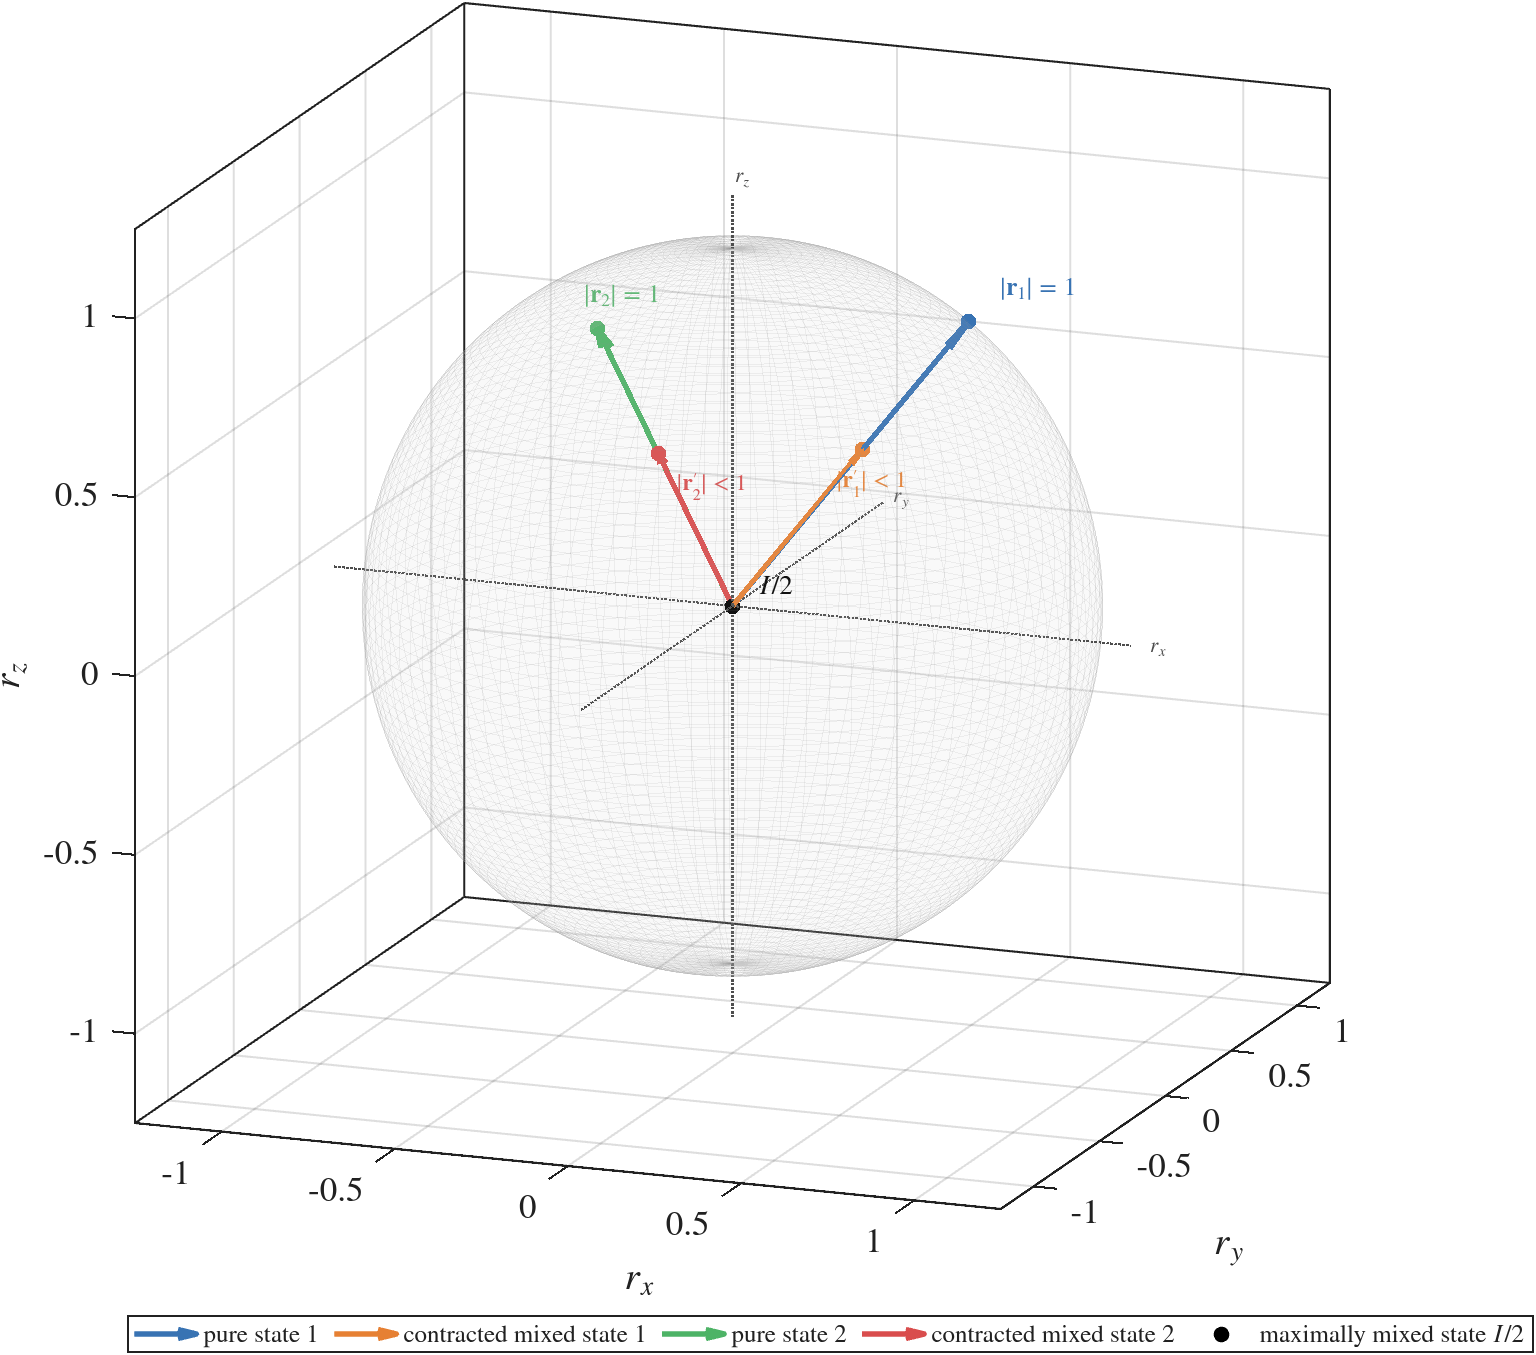
\includegraphics[
        width=0.78\textwidth
    ]{
        figures/theory/bloch_sphere_vector_contraction.png
    }

    \caption{
    Bloch-sphere representation of pure and mixed single-qubit states.
    Pure states lie on the sphere surface and satisfy \( |\mathbf{r}|=1 \), while mixed states are represented by contracted Bloch vectors with \( |\mathbf{r}|<1 \). Statistical averaging and depolarizing mechanisms correspond to contractions toward the center of the Bloch ball.
    }

    \label{fig:bloch_sphere_vector_contraction}
\end{figure}

%========================================================
% SECTION 3.9 — Quantum Channels and Depolarization
%========================================================

\section{Quantum Channels and Depolarization}

The ensemble description introduced in the previous section models statistical fluctuations by averaging over a family of unitary realizations. In that framework, each individual evolution remains coherent, and mixedness originates from classical uncertainty over the applied transformations.

\medskip

More generally, however, a quantum system may interact with additional degrees of freedom that are not observed explicitly. In such cases, the reduced dynamics of the subsystem can no longer be described solely through unitary evolution acting on the state vector. Instead, the evolution must be formulated directly at the level of the density operator.

\medskip

This motivates the introduction of quantum channels, which provide the general mathematical framework for effective non-unitary evolution.

\medskip

\paragraph{Quantum channels.}

A quantum channel is a linear map

\begin{equation}
\mathcal{E}:\rho \mapsto \mathcal{E}(\rho),
\label{eq:quantum_channel_map}
\end{equation}

acting on density operators and satisfying the conditions of complete positivity and trace preservation.

\medskip

A general representation of a quantum channel is given by the operator-sum decomposition

\begin{equation}
\mathcal{E}(\rho)
=
\sum_{\mu}
K_{\mu}
\rho
K_{\mu}^{\dagger},
\qquad
\sum_{\mu}
K_{\mu}^{\dagger}K_{\mu}
=
I,
\label{eq:kraus_operator_sum}
\end{equation}

where the operators \( K_{\mu} \) are referred to as Kraus operators and encode the effective action of the physical process.

\medskip

The channel formalism extends the unitary description introduced previously. While coherent propagation is represented through transformations of the form

\[
\rho
\rightarrow
U \rho U^{\dagger},
\]

more general physical processes may produce irreversible loss of coherence and therefore require a non-unitary reduced description.

\medskip

\paragraph{Global depolarizing channel.}

Among the simplest and most widely used quantum channels is the depolarizing channel, which models isotropic loss of coherence. In the two-qubit setting considered in this work, the global depolarizing model is written as

\begin{equation}
\mathcal{E}_p(\rho)
=
(1-p)\rho
+
\frac{p}{4}I_4,
\label{eq:global_two_qubit_depolarizing_channel}
\end{equation}

where \( I_4 \) denotes the identity operator on the four-dimensional bipartite Hilbert space and \( p \) quantifies the strength of depolarization.

\medskip

This channel continuously interpolates between coherent evolution and complete mixing, providing a simple benchmark model for the study of entanglement degradation and correlation suppression in bipartite systems.

\medskip

\paragraph{Application to Bell states.}

Applying the channel to the Bell state introduced in Eq.~\eqref{eq:bell_psi_plus},

\[
\rho_0
=
|\Psi^+\rangle\langle\Psi^+|,
\]

produces the family of mixed states

\begin{equation}
\rho(p)
=
(1-p)\rho_0
+
\frac{p}{4}I_4.
\label{eq:depolarized_bell_state}
\end{equation}

This construction provides a controlled framework for analyzing the degradation of bipartite quantum correlations under effective noisy evolution.

\bigskip

The global depolarizing model introduced here should be understood as a reference channel rather than as a complete physical model of two-arm fiber propagation. The refinement to independent local depolarizing channels acting on the two propagation arms is developed later in Chapter~\ref{ch:effective_fiber_models}.

%========================================================
% SECTION 3.10 — Computational Representation and Implementation Roadmap
%========================================================

\section{Computational Representation and Implementation Roadmap}

The mathematical structures introduced in this chapter define the computational backbone of the simulator. The purpose of the implementation is not to introduce a separate numerical model, but to realize the theoretical framework in a modular and reproducible form.

\medskip

At MATLAB level, bipartite pure states are represented as \(4 \times 1\) complex vectors and operators acting on the full two-qubit system are represented as \(4 \times 4\) complex matrices.

The computational basis ordering is fixed as

\[
\{|00\rangle, |01\rangle, |10\rangle, |11\rangle\},
\]

and is used consistently across all modules. This convention is critical: tensor products, operator constructions, density matrices, and correlation observables are all defined with respect to this ordering. Any mismatch would lead to incorrect physical results, even if the underlying mathematical expressions are formally correct.

\medskip

State preparation is implemented through dedicated routines returning normalized Bell states in the fixed computational basis. The state \( |\Psi^+\rangle \) is used as the default reference input for the baseline model, providing a controlled benchmark for validating correlation observables, fidelity computations, and entanglement measures under fiber propagation.

\medskip

The fundamental evolution primitive is the tensor-product action

\[
\psi_{\mathrm{out}}
=
(U_A \otimes U_B)\psi_{\mathrm{in}}.
\]

This operation is isolated as a core routine because all unitary propagation models reduce to this structure at the bipartite level. Local single-qubit operators are combined into the global operator \( U_A \otimes U_B \), which is then applied to the input state vector.

\medskip

For the reduced phase model, the simulator is structured around the one-parameter family \( |\psi(\theta)\rangle \). Both parametrizations \( (\theta_A,\theta_B) \) and \( \theta = \theta_A-\theta_B \) are useful: the two-phase representation preserves the physical interpretation of independent fiber arms, while the reduced one-parameter form enables efficient analytical validation and parameter sweeps.

\medskip

The first validated numerical study consists of a parameter sweep in \( \theta \), with numerical evaluation of state vectors, expectation values, and correlation observables. This defines the minimal complete simulation pipeline upon which all subsequent developments are built.

\medskip

For correlation analysis, the simulator evaluates tensor components through the density-operator trace rule

\[
\langle O \rangle = \mathrm{Tr}(\rho O),
\]

using a modular pipeline including:
\begin{itemize}
    \item Pauli operator generation,
    \item tensor-product construction,
    \item expectation-value evaluation,
    \item structured storage of \( T_{ij} \).
\end{itemize}

\medskip

The same computational framework is reused for arbitrary-axis measurements by constructing operators of the form \( \sigma(\mathbf{a}) \otimes \sigma(\mathbf{b}) \), and for CHSH analysis by combining the resulting correlation functions into fixed-axis or optimized Bell parameters.

\medskip

This organization ensures that changes in the physical model, such as stochastic phase evolution, random unitary propagation, or effective quantum channels, can be introduced by modifying well-isolated components while preserving the validated core routines.